% !TEX root = ../my-thesis.tex
%
\chapter{Related Work}
\label{sec:related}

\section{Prior work from Böckenhoff}

The topic of this thesis was built upon the work of many of colleagues at IPP. Daniel Böckenhoff's work in his 2018 paper \cite{Böckenhoff_2018} he demonstrates that artificial neural networks can be used to predict $I_B$, the coil current from the $B$-coils (seen in the following diagram \ref{fig:3}), the from heat load in the experiment. Instead of the divetors that are currently installed on the experiment, the data used was from the prior experimental campaign, which used a limiter \ref{fig:limiter}. A limiter is a piece of graphite designed interface with the plasma to prevent it from interacting with the wall, potentially damaging the wall surface.

\begin{figure}[!htb]
	\centering
	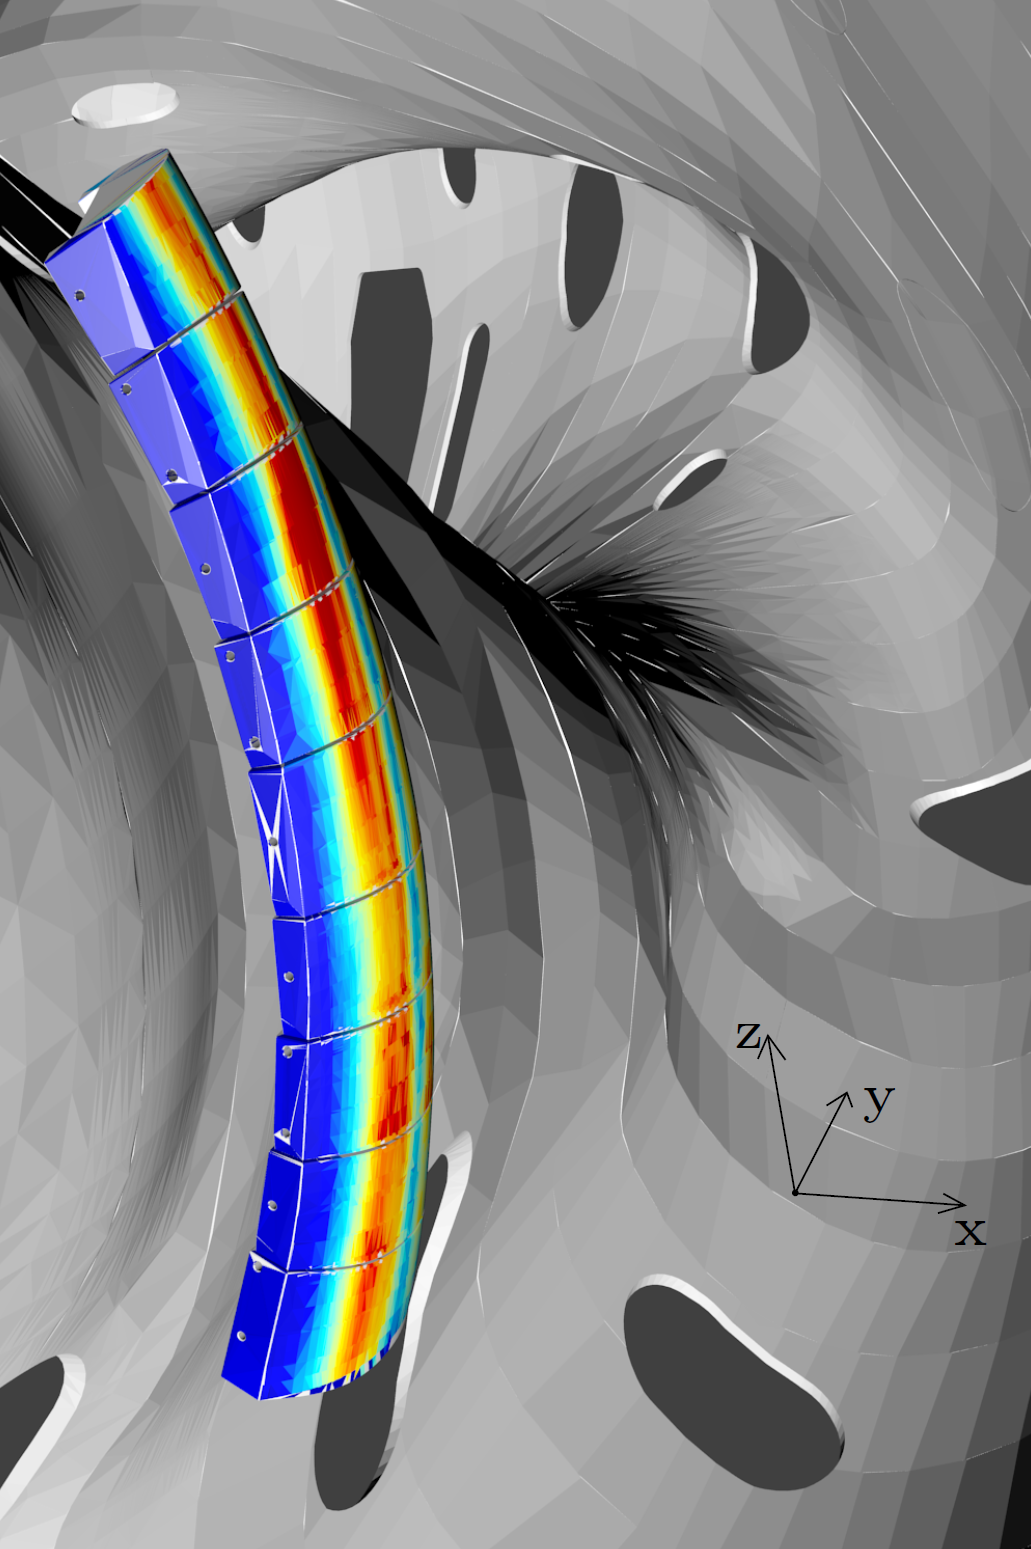
\includegraphics[scale = 0.7]{images/limiter.png}
	\caption{Three-dimensional representation of heat flux on the surface of a limiter in W7X. Taken from \cite{Böckenhoff_2018}} \label{fig:limiter}
\end{figure}

